\chapter{Conclusão}
Este capítulo tem por objetivo expor os resultados alcançados após o desenvolvimento da solução, além de comentar a sua eficácia para a resolução do problema proposto. Ideias de trabalhos futuros também são sugeridas, a fim de incrementar as funcionalidades do sistema desenvolvido e torná-lo mais eficiente.

\section{Resultados}
O sistema desenvolvido foi uma API REST para dar suporte a processos de auditoria para o aplicativo Carteira Digital do Restaurante Universitário da UEA. Para isto, foi feita uma integração com o \emph{back-end} do aplicativo do Restaurante Universitário, possibilitando ao sistema fazer chamadas à API para salvar mensagens de \emph{log}, que são confeccionadas com base no usuário que está se comunicando com o sistema e a interação efetuada por ele.

\begin{figure}
    \centering
    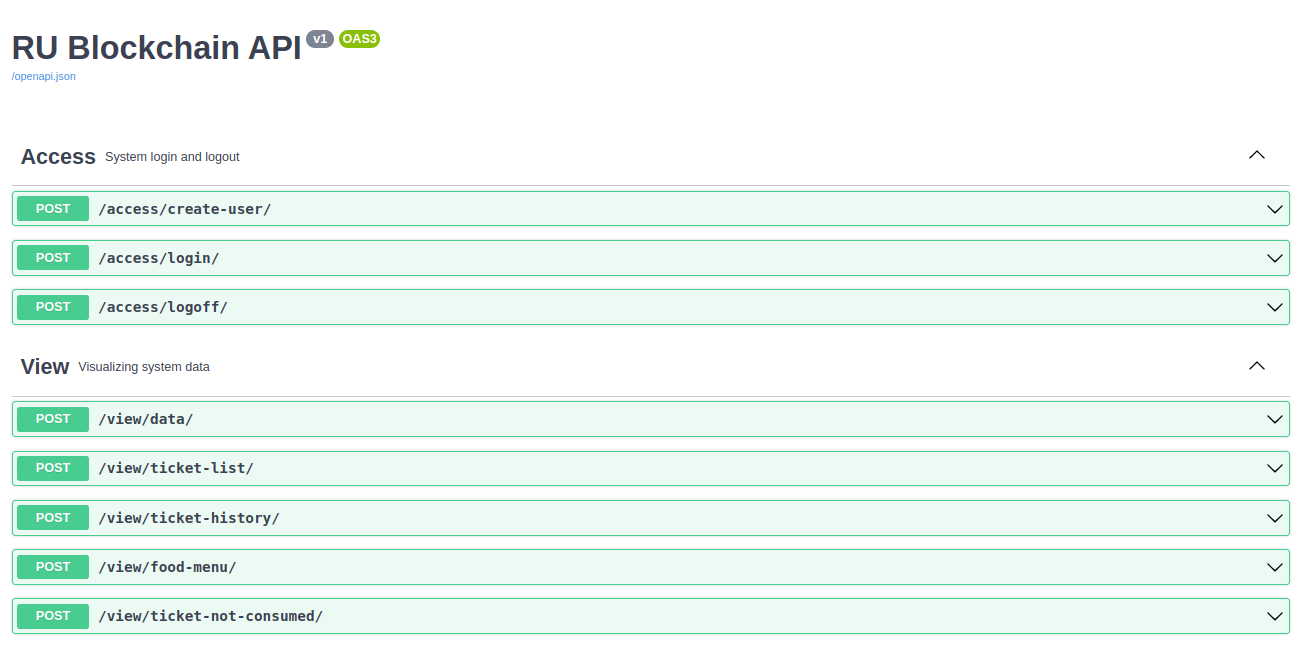
\includegraphics[width=1\textwidth]{img/Cap4/Swagger.png}
    \caption{Parte da página \emph{web} gerada pela documentação OpenAPI}
    \label{fig:openapi}
\end{figure}

A API REST segue a especificação OpenAPI 3.0 (também conhecido como Swagger, em versões anteriores), que define uma interface uniforme, independente de linguagem de programação, para descrever APIs e tornar capaz o seu entendimento tanto por humanos quanto por computadores \cite{openapi_specification}. Com isto, é possível acessar uma página \emph{web} contendo a definição da API REST criada, listando todos os \emph{endpoints} disponíveis, separados por módulo. A Figura \ref{fig:openapi} demonstra parte da documentação gerada pela aplicação. 

Cada um dos \emph{endpoints} da aplicação recebe uma requisição quando o usuário executa a ação relacionada a ele. Se uma pessoa cria um novo usuário, por exemplo, o \emph{back-end} da aplicação do Restaurante Universitário dispara uma requisição para o \emph{endpoint} \emph{/access/create-user/} da Figura \ref{fig:openapi}, enviando os parâmetros necessários para figurar o registro de uma mensagem de \emph{log} na Blockchain.

\begin{figure}
    \centering
    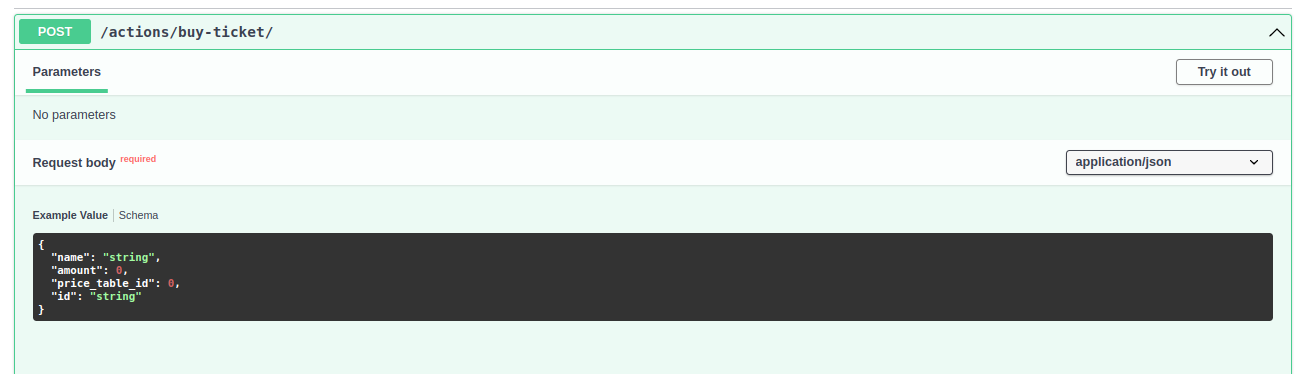
\includegraphics[width=1\textwidth]{img/Cap4/endpoint.png}
    \caption{\emph{Endpoint} para a compra de tickets e seus parâmetros}
    \label{fig:endpoint}
\end{figure}

Os parâmetros utilizados numa requisição podem variar de \emph{endpoint} para \emph{endpoint}. Em geral, todos recebem um valor referente à identificação única do usuário dentro do sistema e, opcionalmente, um valor referente ao nome do usuário. A Figura \ref{fig:endpoint} demonstra os parâmetros necessários para uma requisição de compra de ticket, sendo necessário informar a quantidade de tickets comprados e o id do item comprado a fim de que seja realizado o registro da mensagem.

\begin{figure}
    \centering
    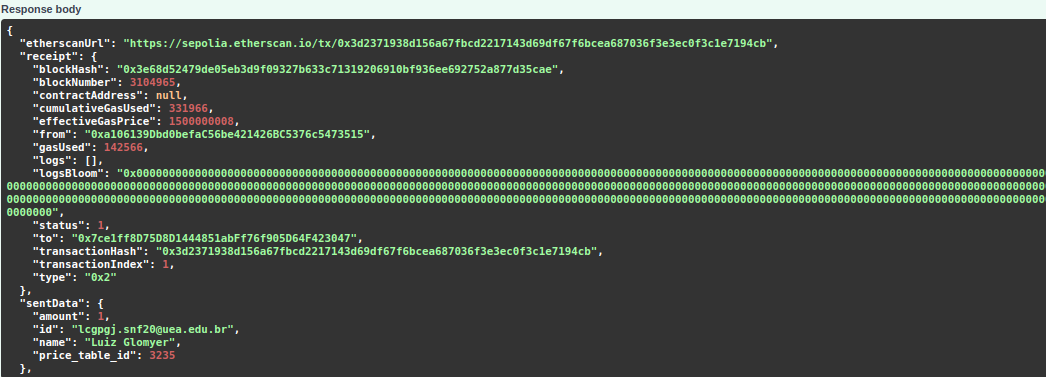
\includegraphics[width=1\textwidth]{img/Cap4/resposta.png}
    \caption{Estrutura da resposta da API após uma requisição}
    \label{fig:resposta}
\end{figure}

Após uma requisição, a mensagem é armazenada na Blockchain, retornando os metadados da transação efetuada, conforme mostra a Figura \ref{fig:resposta}. Informações como o bloco da transação e o seu hash são úteis para confirmar que a transação realmente foi realizada na rede. A partir de seu hash podemos observar mais a fundo as características da transação efetuada com o uso do Etherscan, um \emph{website} que agrega transações feitas na rede. O Etherscan (Figura \ref{fig:etherscan}) permite confirmar se a transação efetuada na rede foi aceita ou rejeitada na Blockchain, além de confirmar se o bloco da transação é um bloco válido ou não. Para isso, a API retorna uma url para a página em questão. Além disso, é retornado também uma cópia dos dados que foram enviados na requisição, agindo como confirmação de que as informações corretas foram utilizadas.


\begin{figure}
    \centering
    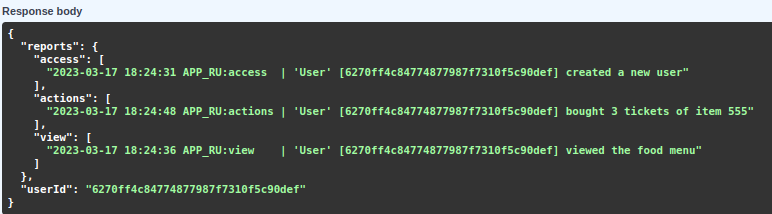
\includegraphics[width=1\textwidth]{img/Cap4/relatorio modulos.png}
    \caption{Visualização de histórico de interações de um usuário, separado por módulos}
    \label{fig:relatorio_modulos}
\end{figure}

\begin{figure}
    \centering
    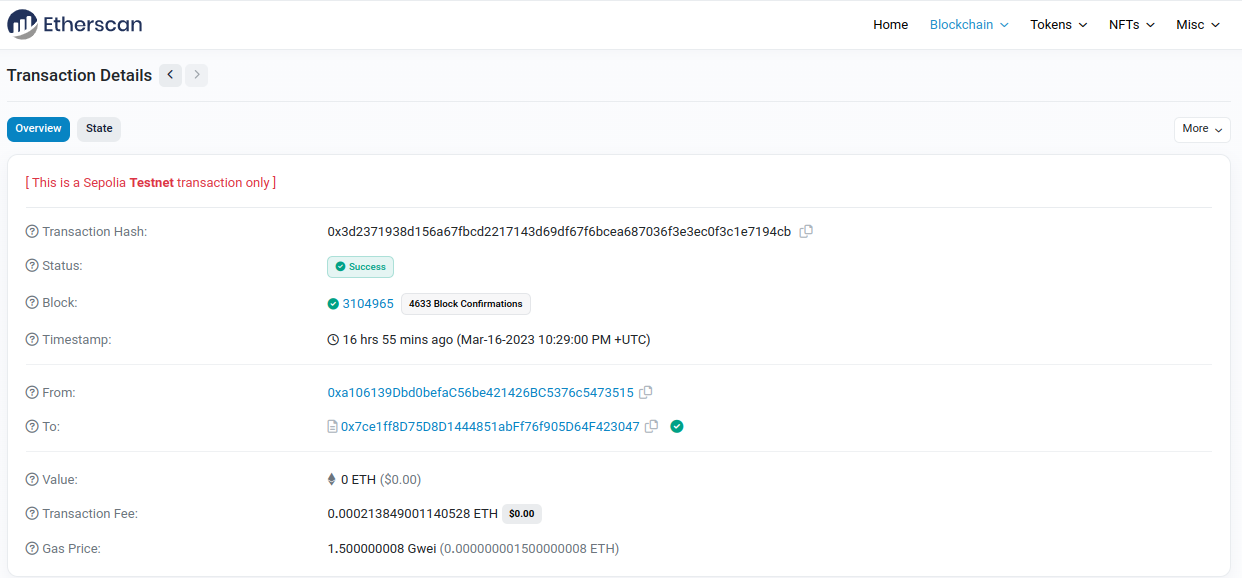
\includegraphics[width=1\textwidth]{img/Cap4/etherscan.png}
    \caption{Detalhes de uma transação via Etherscan}
    \label{fig:etherscan}
\end{figure}

Relatórios de uso do sistema podem ser gerados para usuários específicos por meio de sua identificação única. Existem dois \emph{endpoints} especiais na API que não geram mensagens de \emph{log}, um deles provê uma lista de todos as ações executadas por um usuário no sistema (Figura \ref{fig:trilha_auditoria}) enquanto que o outro lista as ações separadas por módulo. A separação das interações por módulo, conforme demonstrado na Figura \ref{fig:relatorio_modulos}, visa facilitar o processo de auditoria, listando as informações necessárias de acordo com o tipo de interação realizada pelo usuário. Desta forma, cada usuário possui um histórico próprio atrelado à Blockchain, sendo impossível ocorrer qualquer tipo de adulteração nos dados persistidos na rede.


\begin{figure}
    \centering
    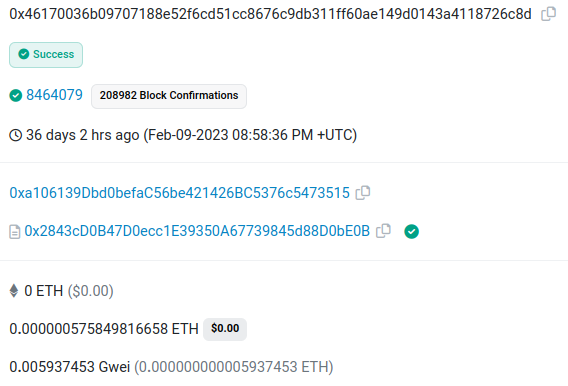
\includegraphics[width=0.45\textwidth]{img/Cap4/tx goerli.png}
    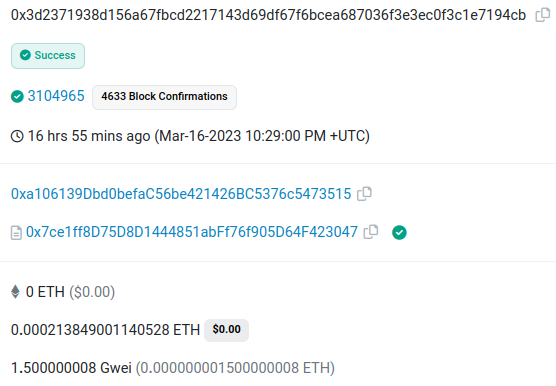
\includegraphics[width=0.45\textwidth]{img/Cap4/tx sepolia.png}
    \caption{Transações realizadas nas \emph{testnets} Goerli e Sepolia, respectivamente}
    \label{fig:preço_transacao}
\end{figure}

Todavia, observou-se que os custos operacionais relacionados a persistência mensagens de \emph{log} podem ser um aspecto impeditivo. Originalmente, a \emph{testnet} utilizada foi a rede Goerli, que possuía custos por transação viáveis; entretanto, durante o desenvolvimento deste trabalho a rede foi considerada como depreciada pelos desenvolvedores da Ethereum, ocasionando uma migração em massa para a rede Sepolia. Além disso, houveram variações no valor da criptomoeda Ether, a encarecendo. Com isto, o preço de \emph{gas} aumentou subitamente, tornando mais alto o preço das transações realizadas pelo sistema. A Figura \ref{fig:preço_transacao} demonstra a discrepância de valores entre as duas \emph{testnets}: supondo a cotação de 1 ETH como equivalente a R\$ 8.000,00, em fevereiro de 2023 o custo médio de uma transação realizada pela API REST custava em torno de R\$ 0,005 na rede Goerli; em março de 2023 uma transação variou de R\$ 1,00 a R\$ 2,50 na rede Sepolia. Isto impacta a viabilidade da solução. Porém, o sistema serviu o seu propósito como prova de conceito, e trabalhos futuros podem ser realizados para estudar métodos com o objetivo de aumentar a viabilidade da solução.

\section{Trabalhos futuros}
Como trabalhos futuros, melhorias ao sistema podem ser implementadas. Otimizações de custo operacional na Blockchain podem ser empregadas com o uso de formas mais sofisticadas de armazenamento de informações na rede, somado também a refatorações no contrato inteligente. Ethereum, por ser uma das redes Blockchain mais bem difundidas e utilizadas, possui taxas de \emph{gas} elevadas se comparada a outras redes Blockchain. Isto se deve a problemas de escalabilidade da plataforma, que pretendem ser sanados após a completa atualização da rede para a Ethereum 2.0. A rede Solana, por exemplo, possui um custo por transação de cerca de \$0.00025 USD por transação \cite{solana_compass}, ao passo que os valores rede Ethereum dependem do tráfego e do volume de transações da rede, podendo ser mais caros. Existem também alternativas livres de custo, como as criptomoedas NANO e TAMA \cite{analytics_insight}. Portanto, existe espaço para otimizar os custos envolvidos ao se executar uma transação na API REST desenvolvida.

Além disso, é possível otimizar o armazenamento de mensagens de \emph{log} salvas na rede. Ao invés de realizar a persistência diretamente no contrato inteligente, pode-se explorar diferentes maneiras de lidar com o fluxo de dados da aplicação. Uma alternativa é utilizar plataformas descentralizadas para armazenamento de arquivos, como o IPFS (InterPlanetary File System). Uma outra abordagem pode ser gerar valores \emph{hash} a partir da mensagem de \emph{log} criada e armazená-los na rede Blockchain, ao passo que a mensagem de \emph{log} em si junto com o \emph{hash} criado são armazenados em um banco de dados, de maneira local ou remota. Otimizar a persistência das mensagens de log é importante pois métodos alternativos têm a possibilidade de serem bem menos dispendiosos em termos de valor de transação e preço de \emph{gas}.

Outro fator importante a ser levado em consideração é a quantidade de informações que são persistidas na rede. O sistema desenvolvido salva toda e qualquer interação realizada pelo usuário dentro do contexto do aplicativo da Carteira Digital do Restaurante Universitário da UEA. É interessante realizar um levantamento acerca de quais são as informações essenciais para serem salvas na rede a fim de que se possa haver processos de auditoria. Dados como registrar que o usuário visualizou a seção de comentários ou o cardápio, por exemplo, podem não ser tão valiosos quando se comparado ao registro de ações-chave no sistema, como a compra de um ticket.